\chapter{Crystals II: Ionic, Covalent and Molecular Solids}\label{ch:b1:crystals-ionic-covalent}

Table salt, crushed, breaks into tiny cubes; a diamond is the hardest
natural material, yet graphite, made of the same carbon atoms, is soft
enough to write with; ice floats on water. All are \omterm{def:b1:crystals-metals:crystal}{crystals}, but their
particles are held together in different ways: ions by electrostatic
attraction, atoms by \omterm{def:b1:lewis-resonance-vsepr:lewis}{covalent bonds}, molecules by the intermolecular
forces of \cref{ch:b1:intermolecular-forces-solvents}. This chapter
applies the cell geometry of the previous chapter to these three families
of solids, and explains, from the sizes of the ions, why sodium chloride
and caesium chloride adopt different structures.

\begin{recall}
A cell's \omterm{def:b1:crystals-metals:multiplicity}{multiplicity}, \omterm{def:b1:crystals-metals:coordination}{coordination number} and \omterm{def:b1:crystals-metals:compactness}{compactness}, and the
octahedral and \omterm{def:b1:crystals-metals:site}{tetrahedral sites} of the \omterm{def:b1:crystals-metals:packings}{face-centred cubic} \omterm{def:b1:crystals-metals:lattice}{lattice}, were
defined in \cref{ch:b1:crystals-metals}; the density of a \omterm{def:b1:crystals-metals:crystal}{crystal} is
$\rho = ZM/(N_A V)$ (\cref{prop:b1:crystals-metals:density}). Ionic radii
were introduced in \cref{def:b1:periodicity:radius}.
\end{recall}

\section{Ionic crystals and radius ratios}

\begin{definition}[Ionic crystal]\label{def:b1:crystals-ionic-covalent:ionic-crystal}
An \emph{ionic crystal}\index{ionic crystal} is a \omterm{def:b1:crystals-metals:crystal}{crystal} of cations and
anions held together by electrostatic attraction. Each ion is surrounded
by ions of opposite charge; the \omterm{def:b1:crystals-metals:crystal}{crystal} is electrically neutral, so the
numbers of cations and anions in a cell are in the ratio of the formula.
\end{definition}

\begin{proposition}[Properties of ionic crystals]\label{prop:b1:crystals-ionic-covalent:ionic-properties}
\omterm{def:b1:crystals-ionic-covalent:ionic-crystal}{Ionic crystals} are hard but brittle (a shift of one layer brings ions of
the same sign face to face, and the \omterm{def:b1:crystals-metals:crystal}{crystal} cleaves), have high melting
points, do not conduct as solids but conduct when molten or dissolved,
and dissolve in \omterm{def:b1:intermolecular-forces-solvents:solvent-classes}{polar solvents} of high permittivity.
\end{proposition}
\admitted

\begin{definition}[Radius ratio]\label{def:b1:crystals-ionic-covalent:radius-ratio}
In an \omterm{def:b1:crystals-ionic-covalent:ionic-crystal}{ionic crystal} of a cation of radius $r_+$ and an anion of radius
$r_-$, the \emph{radius ratio}\index{radius ratio} is $x = r_+/r_-$
(usually $x < 1$, cations being smaller than anions).
\end{definition}

\begin{proposition}[The radius-ratio rule]\label{prop:b1:crystals-ionic-covalent:rule}
In the hard-sphere model, a structure in which each cation touches $n$
anions is stable only if the anions do not touch one another, which
requires $x$ above a limit fixed by the geometry: $x \ge \sqrt3 - 1
\approx 0.732$ for 8 neighbours (cube), $x \ge \sqrt2 - 1 \approx 0.414$
for 6 (octahedron), $x \ge \sqrt{3/2} - 1 \approx 0.225$ for 4
(tetrahedron). The structure adopted is the one of highest coordination
allowed by $x$.
\end{proposition}

\begin{proof}
The cation sits in the hole between $n$ anions in contact with it. At the
limit, the anions also touch one another. Cube: the anions are at the
corners of a cube of edge $2r_-$ and the cation at its centre, so $r_+ +
r_- = \sqrt3\,r_-$. Octahedron: four anions in a square of side $2r_-$,
the cation at its centre, $r_+ + r_- = \sqrt2\,r_-$. Tetrahedron: the
anions at alternate corners of a cube of edge $\sqrt2\,r_-$, the cation at
the centre, $r_+ + r_- = \frac{\sqrt3}{2}\sqrt2\,r_- = \sqrt{3/2}\,r_-$.
Dividing by $r_-$ gives the limits. Below the limit the cation rattles in
a hole too large for it: the anions repel without the attraction being
increased, so a lower coordination, with a smaller hole, is preferred.
\end{proof}

\begin{omfigure}
\begin{tikzpicture}[font=\small, >={Stealth}]
  \draw[->, thick] (0,0) -- (12.4,0) node[right] {$x = r_+/r_-$};
  \foreach \x/\l in {0/0, 2.7/0.225, 4.97/0.414, 8.78/0.732, 12/1} {
    \draw (\x,0.12) -- (\x,-0.12) node[below] {\l};
  }
  \fill[omDef!15] (2.7,0.2) rectangle (4.97,1.0);
  \fill[omProp!15] (4.97,0.2) rectangle (8.78,1.0);
  \fill[omThm!15] (8.78,0.2) rectangle (12,1.0);
  \node[align=center] at (3.83,0.6) {4: ZnS};
  \node[align=center] at (6.87,0.6) {6: NaCl};
  \node[align=center] at (10.4,0.6) {8: CsCl};
  \foreach \x/\l in {3.91/\ce{ZnS}, 6.76/\ce{NaCl}, 10.08/\ce{RbCl}, 11.54/\ce{CsCl}} {
    \draw[omExo, thick] (\x,-0.55) -- (\x,-0.95);
    \node[below, omExo] at (\x,-0.95) {\l};
  }
\end{tikzpicture}

{\small The radius-ratio rule: the \omterm{def:b1:crystals-metals:coordination}{coordination number} of the cation
allowed by $x$, and the measured ratios of four salts (Shannon radii).
Rubidium chloride, at 0.84, should be of the \ce{CsCl} type but adopts
the \ce{NaCl} type: the rule is a guide, not a law
(\cref{exo:b1:crystals-ionic-covalent:12}).}
% ledger: rion:Zn2+IV, rion:S2-VI, rion:Na+VI, rion:Cl-VI, rion:Rb+VI,
% rion:Cs+VIII
\end{omfigure}

\section{Four structure types}

\begin{definition}[Structure types]\label{def:b1:crystals-ionic-covalent:structure-type}
\omterm{def:b1:crystals-ionic-covalent:ionic-crystal}{Ionic crystals} are classified by a few structure types, named after a
representative compound:
\begin{itemize}
  \item \emph{caesium chloride type}\index{caesium chloride type}: anions
        at the corners of a cube, the cation at its centre (8:8);
  \item \emph{rock-salt type}\index{rock-salt type} (sodium chloride
        type): anions on an FCC \omterm{def:b1:crystals-metals:lattice}{lattice}, cations in all its \omterm{def:b1:crystals-metals:site}{octahedral
        sites} (6:6);
  \item \emph{zinc-blende type}\index{zinc-blende type}: anions on an FCC
        \omterm{def:b1:crystals-metals:lattice}{lattice}, cations in half of its \omterm{def:b1:crystals-metals:site}{tetrahedral sites}, one in two in
        alternation (4:4);
  \item \emph{fluorite type}\index{fluorite type}: cations on an FCC
        \omterm{def:b1:crystals-metals:lattice}{lattice}, anions in all its \omterm{def:b1:crystals-metals:site}{tetrahedral sites} (8:4), formula
        \ce{MX2}; in the \emph{antifluorite type}\index{antifluorite type}
        the roles are exchanged (\ce{Li2O}, 4:8).
\end{itemize}
The pair of numbers gives the coordination of the cation and of the
anion.
\end{definition}

\begin{omfigure}
\tdplotsetmaincoords{60}{100}
\begin{tikzpicture}[tdplot_main_coords, font=\small]
  \pic {omcubeo={3}};
    \node[aX={green!55!black}{6.5mm}] at (0,0,0) {};
  \node[aX={violet!70}{3.8mm}] at (0,1.5,0) {};
  \node[aX={green!55!black}{6.5mm}] at (0,3,0) {};
  \node[aX={violet!70}{3.8mm}] at (0,0,1.5) {};
  \node[aX={green!55!black}{6.5mm}] at (0,1.5,1.5) {};
  \node[aX={violet!70}{3.8mm}] at (0,3,1.5) {};
  \node[aX={violet!70}{3.8mm}] at (1.5,0,0) {};
  \node[aX={green!55!black}{6.5mm}] at (0,0,3) {};
  \node[aX={green!55!black}{6.5mm}] at (1.5,1.5,0) {};
  \node[aX={violet!70}{3.8mm}] at (0,1.5,3) {};
  \node[aX={violet!70}{3.8mm}] at (1.5,3,0) {};
  \node[aX={green!55!black}{6.5mm}] at (0,3,3) {};
  \node[aX={green!55!black}{6.5mm}] at (1.5,0,1.5) {};
  \node[aX={violet!70}{3.8mm}] at (1.5,1.5,1.5) {};
  \node[aX={green!55!black}{6.5mm}] at (1.5,3,1.5) {};
  \node[aX={green!55!black}{6.5mm}] at (3,0,0) {};
  \node[aX={violet!70}{3.8mm}] at (1.5,0,3) {};
  \node[aX={violet!70}{3.8mm}] at (3,1.5,0) {};
  \node[aX={green!55!black}{6.5mm}] at (1.5,1.5,3) {};
  \node[aX={green!55!black}{6.5mm}] at (3,3,0) {};
  \node[aX={violet!70}{3.8mm}] at (1.5,3,3) {};
  \node[aX={violet!70}{3.8mm}] at (3,0,1.5) {};
  \node[aX={green!55!black}{6.5mm}] at (3,1.5,1.5) {};
  \node[aX={violet!70}{3.8mm}] at (3,3,1.5) {};
  \node[aX={green!55!black}{6.5mm}] at (3,0,3) {};
  \node[aX={violet!70}{3.8mm}] at (3,1.5,3) {};
  \node[aX={green!55!black}{6.5mm}] at (3,3,3) {};
  \node at (1.5,1.5,-1.75) {\ce{NaCl} (rock salt)};
\end{tikzpicture}
\hspace{1cm}
\begin{tikzpicture}[tdplot_main_coords, font=\small]
  \pic {omcubeo={3}};
    \node[aX={green!55!black}{6.5mm}] at (0,0,0) {};
  \node[aX={green!55!black}{6.5mm}] at (0,3,0) {};
  \node[aX={green!55!black}{6.5mm}] at (0,0,3) {};
  \node[aX={green!55!black}{6.5mm}] at (0,3,3) {};
  \node[aX={blue!60}{7mm}] at (1.5,1.5,1.5) {};
  \node[aX={green!55!black}{6.5mm}] at (3,0,0) {};
  \node[aX={green!55!black}{6.5mm}] at (3,3,0) {};
  \node[aX={green!55!black}{6.5mm}] at (3,0,3) {};
  \node[aX={green!55!black}{6.5mm}] at (3,3,3) {};
  \node at (1.5,1.5,-1.75) {\ce{CsCl}};
\end{tikzpicture}

{\small Left: the rock-salt cell, \ce{Cl-} (green) on an FCC \omterm{def:b1:crystals-metals:lattice}{lattice},
\ce{Na+} (violet) in every \omterm{def:b1:crystals-metals:site}{octahedral site}. Right: the caesium chloride
cell, \ce{Cl-} at the corners, \ce{Cs+} (blue) at the centre. Ions drawn
smaller than in contact.}
\end{omfigure}

\begin{proposition}[Rock-salt and caesium chloride types]\label{prop:b1:crystals-ionic-covalent:nacl-cscl}
In the \omterm{def:b1:crystals-ionic-covalent:structure-type}{rock-salt type}, $Z = 4$ formula units per cell, the ions touch
along an edge, $a = 2(r_+ + r_-)$, and the structure requires $\sqrt2 - 1
\le x$. In the \omterm{def:b1:crystals-ionic-covalent:structure-type}{caesium chloride type}, $Z = 1$, the ions touch along the
main diagonal, $a\sqrt3 = 2(r_+ + r_-)$, and the structure requires
$x \ge \sqrt3 - 1$.
\end{proposition}

\begin{proof}
Rock salt: the anions of the FCC \omterm{def:b1:crystals-metals:lattice}{lattice} count $4$, the cations in the 4
\omterm{def:b1:crystals-metals:site}{octahedral sites} $1 + 12 \times \frac14 = 4$. Along an edge, anion,
cation and anion follow one another in contact. The anions do not overlap
if the face diagonal, which holds three anions of which two touch at
most, satisfies $a\sqrt2 \ge 4r_-$, that is $2(r_+ + r_-)\sqrt2 \ge
4r_-$, or $x \ge \sqrt2 - 1$. Caesium chloride: $8 \times \frac18 = 1$
anion and 1 cation; on the main diagonal, anion, cation, anion in
contact; the anions do not overlap along an edge if $a \ge 2r_-$, that is
$2(r_+ + r_-)/\sqrt3 \ge 2r_-$, or $x \ge \sqrt3 - 1$.
\end{proof}

\begin{example}[Sodium chloride and caesium chloride]\label{ex:b1:crystals-ionic-covalent:nacl}
Sodium chloride has $a = \qty{564.1}{pm}$: $r_+ + r_- = a/2 =
\qty{282.0}{pm}$, against $102 + 181 = \qty{283}{pm}$ from the Shannon
radii; $x = 102/181 = 0.56$, in the octahedral range. Its density is
$\rho = 4 \times 58.44/(6.022 \times 10^{23} \times (5.641 \times
10^{-8})^3) = \qty{2.16}{g/cm^3}$, measured \qty{2.17}{g/cm^3}. Caesium
chloride has $a = \qty{412.3}{pm}$: $r_+ + r_- = a\sqrt3/2 =
\qty{357.1}{pm}$, and $x = 174/181 = 0.96$, in the cubic range.
% ledger: lat:NaCl, rion:Na+VI, rion:Cl-VI, rho:NaCl, lat:CsCl,
% rion:Cs+VIII
\end{example}

\begin{omfigure}
\begin{minipage}[b]{0.31\linewidth}\centering
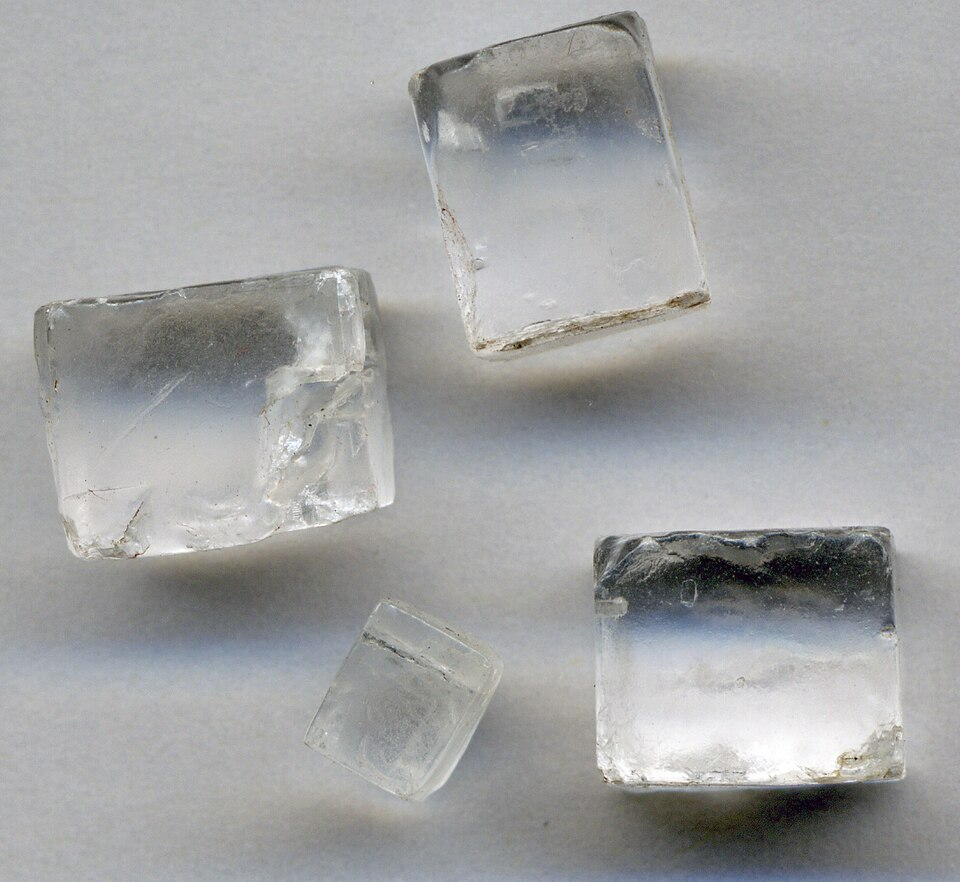
\includegraphics[width=\linewidth]{images/book2/halite.jpg}

{\small Halite (rock salt) \omterm{def:b1:crystals-metals:crystal}{crystals}. Photo: James St. John, CC BY 2.0.}
\end{minipage}\hfill
\begin{minipage}[b]{0.31\linewidth}\centering
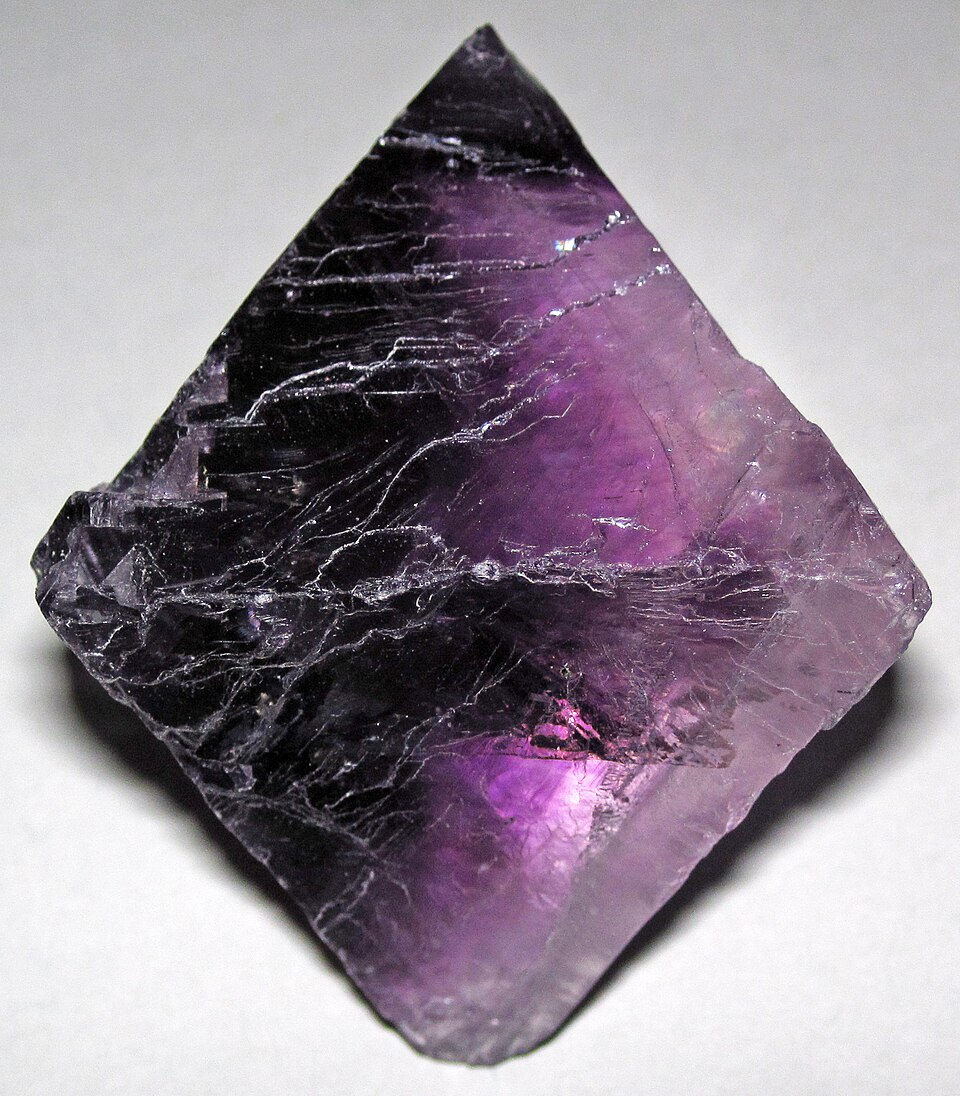
\includegraphics[width=0.85\linewidth]{images/book2/fluorite.jpg}

{\small Fluorite, \ce{CaF2}. Photo: James St. John, CC BY 2.0.}
\end{minipage}\hfill
\begin{minipage}[b]{0.31\linewidth}\centering
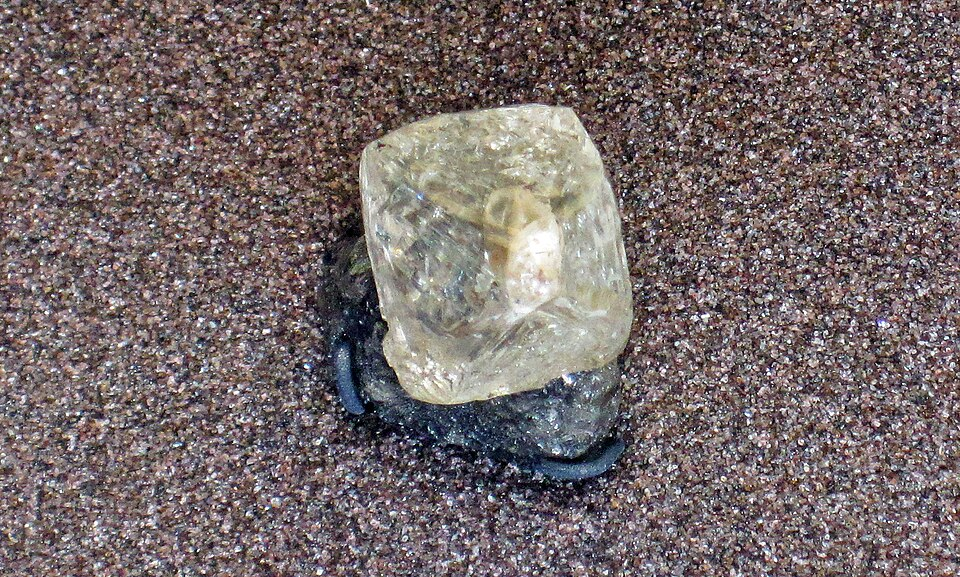
\includegraphics[width=\linewidth]{images/book2/diamond.jpg}

{\small A rough diamond octahedron. Photo: James St. John, CC BY 2.0.}
\end{minipage}
\end{omfigure}

\begin{proposition}[Zinc-blende and fluorite types]\label{prop:b1:crystals-ionic-covalent:zns-caf2}
In the \omterm{def:b1:crystals-ionic-covalent:structure-type}{zinc-blende type}, $Z = 4$, each ion is surrounded by four of the
other kind at the corners of a tetrahedron, and the ions touch along a
quarter of the main diagonal: $a\sqrt3/4 = r_+ + r_-$. In the \omterm{def:b1:crystals-ionic-covalent:structure-type}{fluorite
type}, $Z = 4$ \ce{CaF2} units, each cation has 8 anion neighbours (a cube),
each anion 4 cation neighbours (a tetrahedron), and again $a\sqrt3/4 =
r_+ + r_-$.
\end{proposition}

\begin{proof}
Zinc blende: 4 anions on the FCC \omterm{def:b1:crystals-metals:lattice}{lattice} and 4 cations in half of the 8
\omterm{def:b1:crystals-metals:site}{tetrahedral sites}. A \omterm{def:b1:crystals-metals:site}{tetrahedral site} at $(\frac a4,\frac a4,\frac a4)$
lies at $\frac{a\sqrt3}{4}$ from its four anions. Fluorite: 4 cations and
8 anions in all the \omterm{def:b1:crystals-metals:site}{tetrahedral sites}, ratio $1:2$. The 8 anions inside
the cell form a cube of edge $a/2$, each of whose cubes of anions holds a
cation at the centre of every second one; an anion has its 4 cation
neighbours at $\frac{a\sqrt3}{4}$.
\end{proof}

\begin{omfigure}
\tdplotsetmaincoords{60}{100}
\begin{tikzpicture}[tdplot_main_coords, font=\small]
  \pic {omcubeo={3}};
  \begin{scope}[on background layer]
    \draw[black!45, line width=1.2pt] (0.75,0.75,2.25) -- (0,0,3) (0.75,0.75,2.25) -- (0,1.5,1.5) (0.75,0.75,2.25) -- (1.5,0,1.5) (0.75,0.75,2.25) -- (1.5,1.5,3) (0.75,2.25,0.75) -- (0,1.5,1.5) (0.75,2.25,0.75) -- (0,3,0) (0.75,2.25,0.75) -- (1.5,1.5,0) (0.75,2.25,0.75) -- (1.5,3,1.5) (2.25,0.75,0.75) -- (1.5,0,1.5) (2.25,0.75,0.75) -- (1.5,1.5,0) (2.25,0.75,0.75) -- (3,0,0) (2.25,0.75,0.75) -- (3,1.5,1.5) (2.25,2.25,2.25) -- (1.5,1.5,3) (2.25,2.25,2.25) -- (1.5,3,1.5) (2.25,2.25,2.25) -- (3,1.5,1.5) (2.25,2.25,2.25) -- (3,3,3);
  \end{scope}
    \node[aX={yellow!75!orange}{6mm}] at (0,0,0) {};
  \node[aX={yellow!75!orange}{6mm}] at (0,3,0) {};
  \node[aX={yellow!75!orange}{6mm}] at (0,1.5,1.5) {};
  \node[aX={gray!60}{3.6mm}] at (0.75,2.25,0.75) {};
  \node[aX={yellow!75!orange}{6mm}] at (0,0,3) {};
  \node[aX={yellow!75!orange}{6mm}] at (1.5,1.5,0) {};
  \node[aX={gray!60}{3.6mm}] at (0.75,0.75,2.25) {};
  \node[aX={yellow!75!orange}{6mm}] at (0,3,3) {};
  \node[aX={yellow!75!orange}{6mm}] at (1.5,0,1.5) {};
  \node[aX={gray!60}{3.6mm}] at (2.25,0.75,0.75) {};
  \node[aX={yellow!75!orange}{6mm}] at (1.5,3,1.5) {};
  \node[aX={yellow!75!orange}{6mm}] at (3,0,0) {};
  \node[aX={yellow!75!orange}{6mm}] at (1.5,1.5,3) {};
  \node[aX={yellow!75!orange}{6mm}] at (3,3,0) {};
  \node[aX={gray!60}{3.6mm}] at (2.25,2.25,2.25) {};
  \node[aX={yellow!75!orange}{6mm}] at (3,1.5,1.5) {};
  \node[aX={yellow!75!orange}{6mm}] at (3,0,3) {};
  \node[aX={yellow!75!orange}{6mm}] at (3,3,3) {};
  \node at (1.5,1.5,-1.75) {\ce{ZnS} (zinc blende)};
\end{tikzpicture}
\hspace{1cm}
\begin{tikzpicture}[tdplot_main_coords, font=\small]
  \pic {omcubeo={3}};
    \node[aX={green!35!gray}{4.4mm}] at (0,0,0) {};
  \node[aX={green!35!gray}{4.4mm}] at (0,3,0) {};
  \node[aX={green!35!gray}{4.4mm}] at (0,1.5,1.5) {};
  \node[aX={green!45!yellow}{5.0mm}] at (0.75,0.75,0.75) {};
  \node[aX={green!45!yellow}{5.0mm}] at (0.75,2.25,0.75) {};
  \node[aX={green!35!gray}{4.4mm}] at (0,0,3) {};
  \node[aX={green!35!gray}{4.4mm}] at (1.5,1.5,0) {};
  \node[aX={green!45!yellow}{5.0mm}] at (0.75,0.75,2.25) {};
  \node[aX={green!35!gray}{4.4mm}] at (0,3,3) {};
  \node[aX={green!35!gray}{4.4mm}] at (1.5,0,1.5) {};
  \node[aX={green!45!yellow}{5.0mm}] at (0.75,2.25,2.25) {};
  \node[aX={green!45!yellow}{5.0mm}] at (2.25,0.75,0.75) {};
  \node[aX={green!35!gray}{4.4mm}] at (1.5,3,1.5) {};
  \node[aX={green!35!gray}{4.4mm}] at (3,0,0) {};
  \node[aX={green!45!yellow}{5.0mm}] at (2.25,2.25,0.75) {};
  \node[aX={green!35!gray}{4.4mm}] at (1.5,1.5,3) {};
  \node[aX={green!35!gray}{4.4mm}] at (3,3,0) {};
  \node[aX={green!45!yellow}{5.0mm}] at (2.25,0.75,2.25) {};
  \node[aX={green!45!yellow}{5.0mm}] at (2.25,2.25,2.25) {};
  \node[aX={green!35!gray}{4.4mm}] at (3,1.5,1.5) {};
  \node[aX={green!35!gray}{4.4mm}] at (3,0,3) {};
  \node[aX={green!35!gray}{4.4mm}] at (3,3,3) {};
  \node at (1.5,1.5,-1.75) {\ce{CaF2} (fluorite)};
\end{tikzpicture}

{\small Left: zinc blende, \ce{S^{2-}} (yellow) on an FCC \omterm{def:b1:crystals-metals:lattice}{lattice} and
\ce{Zn^{2+}} (grey) in alternate \omterm{def:b1:crystals-metals:site}{tetrahedral sites}, each joined to its
four neighbours. Right: fluorite, \ce{Ca^{2+}} (grey-green) on an FCC
\omterm{def:b1:crystals-metals:lattice}{lattice} and \ce{F-} (light green) in all eight \omterm{def:b1:crystals-metals:site}{tetrahedral sites}.}
\end{omfigure}

\begin{example}[Zinc blende and fluorite]\label{ex:b1:crystals-ionic-covalent:zns}
Zinc blende has $a = \qty{540.9}{pm}$: $r_+ + r_- = a\sqrt3/4 =
\qty{234.2}{pm}$ (Shannon: $60 + 184 = \qty{244}{pm}$, the sulfide radius
being tabulated only for six neighbours), and $x = 60/184 = 0.33$, in the
tetrahedral range. Fluorite has $a = \qty{546.3}{pm}$: $r_+ + r_- =
\qty{236.6}{pm}$ (Shannon $112 + 131 = \qty{243}{pm}$), and $x = 0.85$:
the cation sits in a cube of 8 anions, as the rule demands.
% ledger: lat:ZnS, rion:Zn2+IV, rion:S2-VI, lat:CaF2, rion:Ca2+VIII,
% rion:F-IV
\end{example}

\begin{method}[Predicting a structure]\label{met:b1:crystals-ionic-covalent:predict}
To predict the structure of an ionic compound \ce{MX} or \ce{MX2}:
\begin{enumerate}
  \item compute $x = r_+/r_-$ from tabulated radii (for the expected
        coordination);
  \item read the coordination of the cation from the radius-ratio rule;
  \item choose the type that has this coordination and the right formula:
        \ce{MX} with 8: \ce{CsCl}; with 6: \ce{NaCl}; with 4: zinc blende;
        \ce{MX2} with 8: fluorite;
  \item check against the measured \omterm{def:b1:crystals-metals:lattice}{lattice} parameter; remember that
        polarisable ions (\ce{S^{2-}}, \ce{I-}) and small, charged cations
        give bonds partly covalent, for which the rule fails.
\end{enumerate}
\end{method}

\section{Covalent crystals}

\begin{definition}[Covalent crystal]\label{def:b1:crystals-ionic-covalent:covalent-crystal}
A \emph{covalent crystal}\index{covalent crystal} (or network solid) is a
\omterm{def:b1:crystals-metals:crystal}{crystal} in which all the atoms are linked by \omterm{def:b1:lewis-resonance-vsepr:lewis}{covalent bonds} into one
giant molecule: diamond, silicon, quartz \ce{SiO2}. In a layered
covalent \omterm{def:b1:crystals-metals:crystal}{crystal} such as graphite, the covalent network extends only in
planes, which are held to one another by \omterm{def:b1:intermolecular-forces-solvents:vdw}{van der Waals interactions}.
\end{definition}

\begin{proposition}[The diamond structure]\label{prop:b1:crystals-ionic-covalent:diamond}
In diamond the carbon atoms occupy the FCC \omterm{def:b1:crystals-metals:lattice}{lattice} and half of its
\omterm{def:b1:crystals-metals:site}{tetrahedral sites}, as the two kinds of ions of zinc blende: $Z = 8$, each
carbon bonded to four others at the corners of a tetrahedron, at the
distance $a\sqrt3/4$. For touching spheres the \omterm{def:b1:crystals-metals:compactness}{compactness} is
\[
  C = \frac{\pi\sqrt3}{16} \approx 0.34 .
\]
\end{proposition}

\begin{proof}
$Z = 4 + 4 = 8$. Neighbouring atoms touch: $2R = a\sqrt3/4$, so $a =
8R/\sqrt3$ and $C = 8 \cdot \frac43\pi R^3/a^3 = \frac{32}{3}\pi R^3 \cdot
\frac{3\sqrt3}{512 R^3} = \frac{\pi\sqrt3}{16}$.
\end{proof}

\begin{omfigure}
\tdplotsetmaincoords{60}{100}
\begin{tikzpicture}[tdplot_main_coords, font=\small]
  \pic {omcubeo={3}};
  \begin{scope}[on background layer]
    \draw[black!55, line width=1.4pt] (0.75,0.75,2.25) -- (0,0,3) (0.75,0.75,2.25) -- (0,1.5,1.5) (0.75,0.75,2.25) -- (1.5,0,1.5) (0.75,0.75,2.25) -- (1.5,1.5,3) (0.75,2.25,0.75) -- (0,1.5,1.5) (0.75,2.25,0.75) -- (0,3,0) (0.75,2.25,0.75) -- (1.5,1.5,0) (0.75,2.25,0.75) -- (1.5,3,1.5) (2.25,0.75,0.75) -- (1.5,0,1.5) (2.25,0.75,0.75) -- (1.5,1.5,0) (2.25,0.75,0.75) -- (3,0,0) (2.25,0.75,0.75) -- (3,1.5,1.5) (2.25,2.25,2.25) -- (1.5,1.5,3) (2.25,2.25,2.25) -- (1.5,3,1.5) (2.25,2.25,2.25) -- (3,1.5,1.5) (2.25,2.25,2.25) -- (3,3,3);
  \end{scope}
  \node[aX={black!65}{3.6mm}] at (0,0,0) {};
  \node[aX={black!65}{3.6mm}] at (0,3,0) {};
  \node[aX={black!65}{3.6mm}] at (0,1.5,1.5) {};
  \node[aX={black!65}{3.6mm}] at (0.75,2.25,0.75) {};
  \node[aX={black!65}{3.6mm}] at (0,0,3) {};
  \node[aX={black!65}{3.6mm}] at (1.5,1.5,0) {};
  \node[aX={black!65}{3.6mm}] at (0.75,0.75,2.25) {};
  \node[aX={black!65}{3.6mm}] at (0,3,3) {};
  \node[aX={black!65}{3.6mm}] at (1.5,0,1.5) {};
  \node[aX={black!65}{3.6mm}] at (2.25,0.75,0.75) {};
  \node[aX={black!65}{3.6mm}] at (1.5,3,1.5) {};
  \node[aX={black!65}{3.6mm}] at (3,0,0) {};
  \node[aX={black!65}{3.6mm}] at (1.5,1.5,3) {};
  \node[aX={black!65}{3.6mm}] at (3,3,0) {};
  \node[aX={black!65}{3.6mm}] at (2.25,2.25,2.25) {};
  \node[aX={black!65}{3.6mm}] at (3,1.5,1.5) {};
  \node[aX={black!65}{3.6mm}] at (3,0,3) {};
  \node[aX={black!65}{3.6mm}] at (3,3,3) {};
  \node at (1.5,1.5,-1.75) {diamond};
\end{tikzpicture}
\hspace{0.8cm}
\begin{tikzpicture}[font=\small, y={(0cm,0.45cm)}, z={(0cm,1cm)}, x={(1cm,0cm)}]
  % two honeycomb layers seen in perspective, ABAB stacking
  \foreach \zz/\dy/\col in {0/0/black!40, 1.7/0.82/black!80} {
    \foreach \i in {0,1,2} \foreach \j in {0,1} {
      \pgfmathsetmacro\cx{1.42*\i+0.71*\j}
      \pgfmathsetmacro\cy{1.23*\j+\dy}
      \foreach \k in {0,60,...,300} {
        \pgfmathsetmacro\ka{\k+60}
        \draw[\col, line width=1pt] ({\cx+0.82*cos(\k+30)},{\cy+0.82*sin(\k+30)},\zz)
          -- ({\cx+0.82*cos(\ka+30)},{\cy+0.82*sin(\ka+30)},\zz);
      }
    }
  }
  \draw[<->, omThm] (5.6,0.9,0) -- (5.6,0.9,1.7) node[midway, right] {\qty{335}{pm}};
  \node at (2.4,-1.6,0) {graphite};
\end{tikzpicture}

{\small Left: the diamond cell, each carbon bonded to four others in a
tetrahedron. Right: graphite, layers of hexagons (C--C \qty{141.8}{pm}
within a layer) stacked \qty{334.8}{pm} apart, held by London forces; the
layers alternate ABAB.}
% ledger: lat:C-graphite.a, lat:C-graphite.c (C-C = a/sqrt3; interlayer = c/2)
\end{omfigure}

\begin{example}[Diamond, silicon, graphite]\label{ex:b1:crystals-ionic-covalent:carbon}
Diamond has $a = \qty{356.7}{pm}$: \ce{C-C} $= a\sqrt3/4 =
\qty{154.5}{pm}$, the single bond of ethane, and $\rho =
\qty{3.52}{g/cm^3}$. Silicon, of the same structure with $a =
\qty{543.1}{pm}$, has \ce{Si-Si} $= \qty{235.2}{pm}$ and $\rho =
\qty{2.33}{g/cm^3}$ (measured 2.33). In graphite each carbon is bonded
to three others in a plane at \qty{141.8}{pm}, a bond order between one
and two (resonance over the layer), while the layers are
\qty{334.8}{pm} apart. Diamond, rigid in three dimensions, is the hardest
natural material and an insulator; graphite cleaves between its layers,
which slide easily, and conducts electricity within them through its
delocalised $\pi$ electrons.
% ledger: lat:C-diamond, lat:Si, rho:Si, lat:C-graphite.a, lat:C-graphite.c,
% geo:C2H6.rCC
\end{example}

\begin{omfigure}
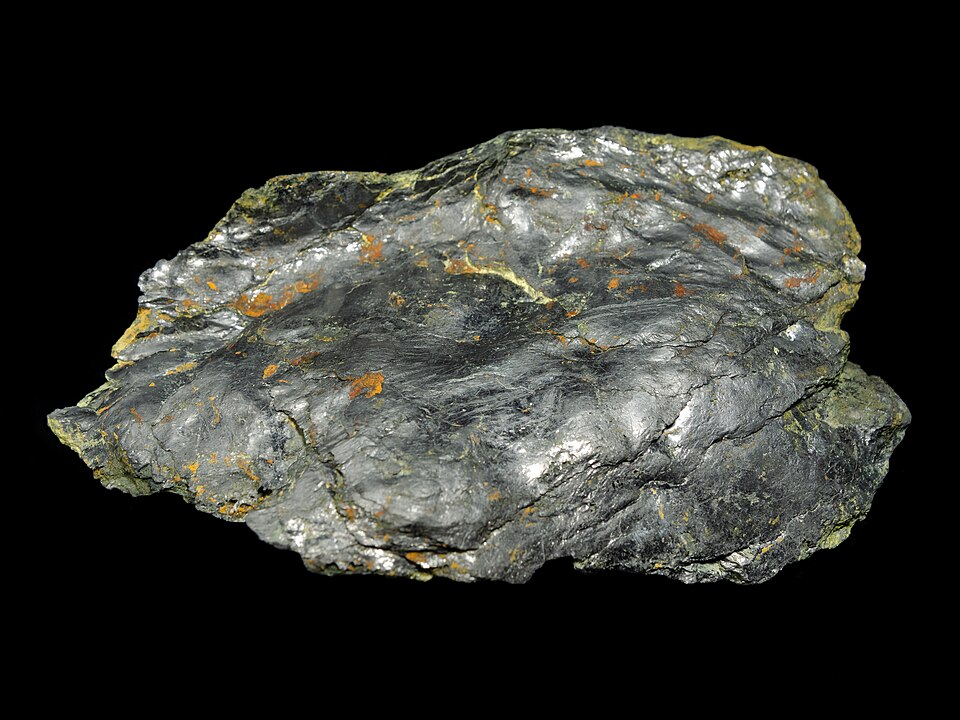
\includegraphics[width=0.36\linewidth]{images/book2/graphite.jpg}

{\small A specimen of natural graphite, with its metallic lustre. Photo:
Zbynek Burival, CC BY-SA 4.0.}
\end{omfigure}

\section{Molecular crystals}

\begin{definition}[Molecular crystal]\label{def:b1:crystals-ionic-covalent:molecular-crystal}
A \emph{molecular crystal}\index{molecular crystal} is a \omterm{def:b1:crystals-metals:crystal}{crystal} of
molecules held together by intermolecular forces --- \omterm{def:b1:intermolecular-forces-solvents:vdw}{van der Waals
interactions} and, if possible, \omterm{def:b1:intermolecular-forces-solvents:hbond}{hydrogen bonds} --- while each molecule
keeps its own \omterm{def:b1:lewis-resonance-vsepr:lewis}{covalent bonds}: diiodine, dry ice \ce{CO2(s)}, ice, sugar.
\end{definition}

\begin{proposition}[Properties of molecular crystals]\label{prop:b1:crystals-ionic-covalent:molecular}
\omterm{def:b1:crystals-ionic-covalent:molecular-crystal}{Molecular crystals} are soft and melt or sublime at low temperatures,
since only weak intermolecular forces are broken; they do not conduct.
\end{proposition}
\admitted

\begin{example}[Ice]\label{ex:b1:crystals-ionic-covalent:ice}
In ordinary ice each water molecule is hydrogen-bonded to four others at
the corners of a tetrahedron: two by its own hydrogens and two by its
\omterm{def:b1:lewis-resonance-vsepr:lewis}{lone pairs}. This open, hexagonal network, imposed by the directions of
the \omterm{def:b1:intermolecular-forces-solvents:hbond}{hydrogen bonds}, leaves much empty space: ice is less dense than liquid
water, in which the network is partly broken and the molecules come
closer. The hexagonal symmetry of the network shows in the six-fold shape
of snow \omterm{def:b1:crystals-metals:crystal}{crystals}.
\end{example}

\begin{omfigure}
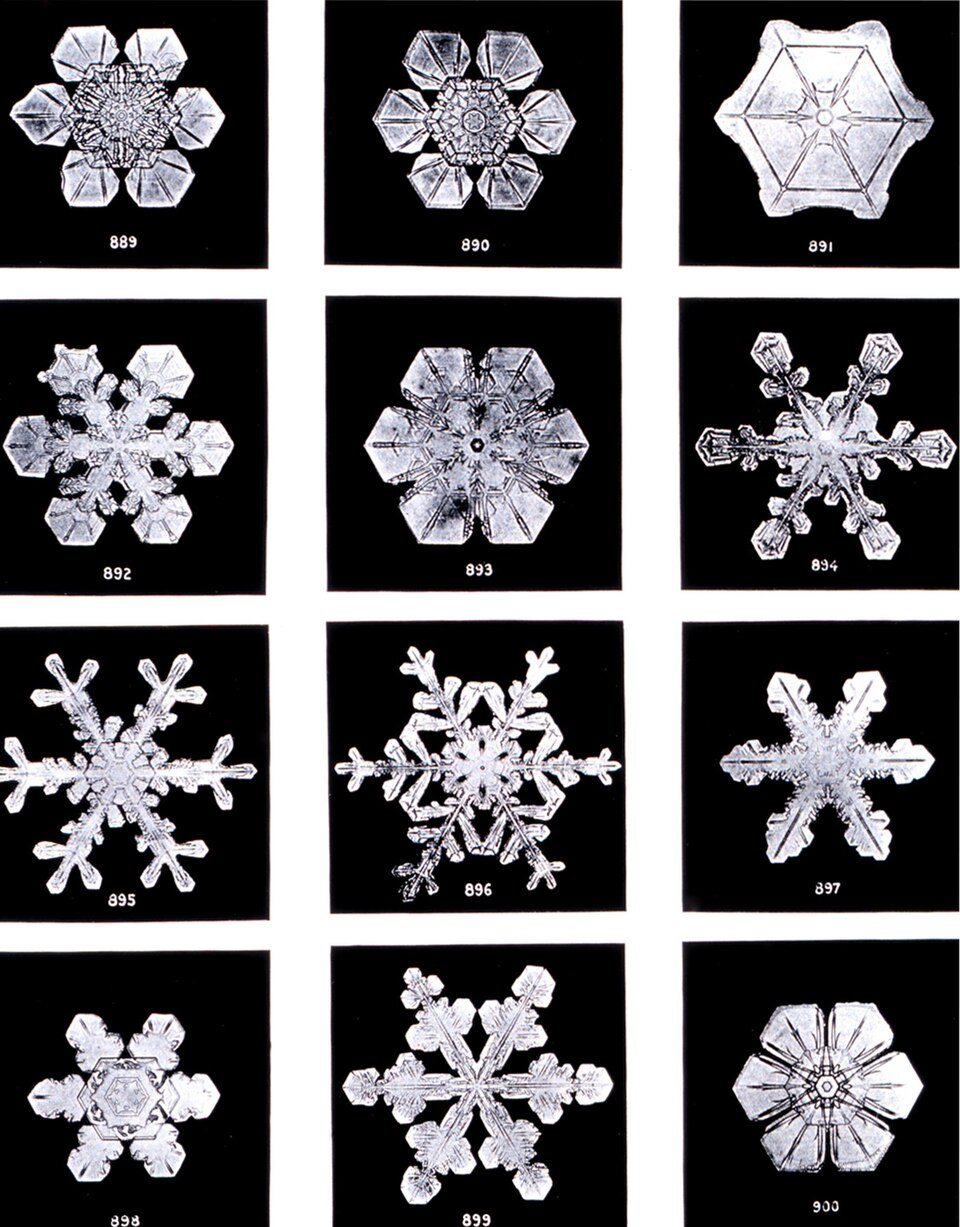
\includegraphics[width=0.38\linewidth]{images/book2/bentley-snowflakes.jpg}

{\small Snow \omterm{def:b1:crystals-metals:crystal}{crystals} photographed by Wilson Bentley about 1902: every one
has six-fold symmetry, the trace of the hexagonal network of \omterm{def:b1:intermolecular-forces-solvents:hbond}{hydrogen
bonds} in ice. Public domain.}
\end{omfigure}

\section{Comparing the four kinds of solids}

\begin{center}
\small
\begin{tabular}{lllll}
\hline
solid & particles & cohesion & properties & examples \\
\hline
metallic & cations, electrons & \omterm{def:b1:crystals-metals:metallic-bond}{metallic bond} & conductor, ductile & \ce{Cu}, \ce{Fe}, \ce{Na} \\
ionic & cations, anions & electrostatic & hard, brittle, insulating & \ce{NaCl}, \ce{CaF2} \\
covalent & atoms & \omterm{def:b1:lewis-resonance-vsepr:lewis}{covalent bonds} & very hard, high melting & diamond, \ce{SiO2} \\
molecular & molecules & van der Waals, H bonds & soft, low melting & \ce{I2}, ice \\
\hline
\end{tabular}
\end{center}

\begin{remark}[A continuum]\label{rem:b1:crystals-ionic-covalent:continuum}
The classes are idealisations. Zinc sulfide has bonds partly ionic,
partly covalent, which is why its sulfide--zinc distance is shorter than
the sum of the ionic radii; graphite is covalent in its layers and
molecular between them. The \omterm{def:b1:periodicity:electronegativity}{electronegativity} difference
(\cref{prop:b1:periodicity:en-trend}) is the guide: the larger it is, the
more ionic the solid.
\end{remark}

\section{Exercises}

\begin{exercise}[$\star$]\label{exo:b1:crystals-ionic-covalent:1}
In the rock-salt cell, count the cations and the anions, give the
coordination of each, and check that the formula \ce{NaCl} is respected.
\end{exercise}

\begin{exercise}[$\star$]\label{exo:b1:crystals-ionic-covalent:2}
Caesium chloride has $a = \qty{412.3}{pm}$. Compute the shortest
\ce{Cs-Cl} distance and the number of formula units per cell.
\end{exercise}

\begin{exercise}[$\star$]\label{exo:b1:crystals-ionic-covalent:3}
Using the radii $r(\ce{Na+}) = \qty{102}{pm}$ and $r(\ce{Cl-}) =
\qty{181}{pm}$, compute the \omterm{def:b1:crystals-ionic-covalent:radius-ratio}{radius ratio} of \ce{NaCl} and predict the
coordination of the cation.
\end{exercise}

\begin{exercise}[$\star$]\label{exo:b1:crystals-ionic-covalent:4}
Classify as metallic, ionic, covalent or molecular: copper, sodium
chloride, diamond, diiodine, quartz \ce{SiO2}, ice, calcium fluoride.
\end{exercise}

\begin{exercise}[$\star\star$]\label{exo:b1:crystals-ionic-covalent:5}
Prove that the rock-salt structure requires $r_+/r_- \ge \sqrt2 - 1$.
\end{exercise}

\begin{exercise}[$\star\star$]\label{exo:b1:crystals-ionic-covalent:6}
Compute the density of sodium chloride from $a = \qty{564.1}{pm}$
($M(\ce{NaCl}) = \qty{58.44}{g/mol}$) and compare with
\qty{2.17}{g/cm^3}.
\end{exercise}

\begin{exercise}[$\star\star$]\label{exo:b1:crystals-ionic-covalent:7}
Compute the density of caesium chloride ($M = \qty{168.36}{g/mol}$,
$a = \qty{412.3}{pm}$) and compare with the measured \qty{3.99}{g/cm^3}.
% ledger: rho:CsCl
\end{exercise}

\begin{exercise}[$\star\star$]\label{exo:b1:crystals-ionic-covalent:8}
For zinc blende ($a = \qty{540.9}{pm}$, $M = \qty{97.44}{g/mol}$) compute
the \ce{Zn-S} distance and the density, and compare with the measured
\qty{4.04}{g/cm^3}.
% ledger: rho:ZnS
\end{exercise}

\begin{exercise}[$\star\star$]\label{exo:b1:crystals-ionic-covalent:9}
Graphite has a hexagonal cell with $a = \qty{245.6}{pm}$ and
$c = \qty{669.6}{pm}$, containing 4 atoms. Compute the \ce{C-C} distance
in a layer ($a/\sqrt3$), the distance between layers ($c/2$) and the
density. Why is graphite less dense than diamond?
\end{exercise}

\begin{exercise}[$\star\star\star$]\label{exo:b1:crystals-ionic-covalent:10}
Prove that the \omterm{def:b1:crystals-metals:compactness}{compactness} of diamond is $\pi\sqrt3/16$, and explain why
the hardest material is one of the least compact.
\end{exercise}

\begin{exercise}[$\star\star\star$]\label{exo:b1:crystals-ionic-covalent:11}
Silicon has the diamond structure with $a = \qty{543.1}{pm}$. Compute
the \ce{Si-Si} bond length, the \omterm{def:b1:periodicity:radius}{covalent radius} of silicon and the
density ($M = \qty{28.09}{g/mol}$); compare with \qty{2.33}{g/cm^3}.
\end{exercise}

\begin{exercise}[$\star\star\star$]\label{exo:b1:crystals-ionic-covalent:12}
Rubidium chloride has $r(\ce{Rb+}) = \qty{152}{pm}$ (six neighbours) and
$r(\ce{Cl-}) = \qty{181}{pm}$. Which structure does the radius-ratio rule
predict? Under ordinary conditions it is of the \omterm{def:b1:crystals-ionic-covalent:structure-type}{rock-salt type} with
$a = \qty{658.1}{pm}$: check the \ce{Rb-Cl} distance, and suggest why the
rule fails here.
% ledger: rion:Rb+VI, rion:Cl-VI, lat:RbCl
\end{exercise}

\section{Problem: Fluorite, the Mineral and the Lens}

\begin{problem}[{Weekend problem --- the fluorite cell, its \omterm{def:b1:crystals-ionic-covalent:radius-ratio}{radius ratio},
two relatives (\ce{Li2O} and diamond), and the density of fluorite
computed from its cell}]
\label{pb:b1:crystals-ionic-covalent:1}
Fluorite, \ce{CaF2}, is a mineral; grown as large clear \omterm{def:b1:crystals-metals:crystal}{crystals} it makes
lenses that transmit ultraviolet light. Its cell is cubic, $a =
\qty{546.3}{pm}$; \ce{Ca^{2+}} on an FCC \omterm{def:b1:crystals-metals:lattice}{lattice}, \ce{F-} in the
\omterm{def:b1:crystals-metals:site}{tetrahedral sites}. Radii: $r(\ce{Ca^{2+}}) = \qty{112}{pm}$ (eight
neighbours), $r(\ce{F-}) = \qty{131}{pm}$ (four neighbours). Molar masses
(g/mol): \ce{Ca} 40.08, \ce{F} 19.00, \ce{Li} 6.94, \ce{O} 16.00, \ce{C}
12.01, \ce{Si} 28.09; $N_A = \qty{6.022e23}{mol^{-1}}$.
% ledger: lat:CaF2, rion:Ca2+VIII, rion:F-IV, aw:Ca, aw:F, aw:Li, aw:O,
% aw:C, aw:Si, const:NA

\medskip
\noindent\textbf{Part I --- The cell.}
\begin{enumerate}
  \item Give the positions of the \ce{Ca^{2+}} ions in the cell and count
        them.
  \item How many \omterm{def:b1:crystals-metals:site}{tetrahedral sites} does the cell contain? Deduce the
        number of \ce{F-} ions and check the formula.
  \item What is the coordination of \ce{F-}? Of \ce{Ca^{2+}}?
  \item Compute the shortest \ce{Ca-F} distance.
  \item Compare it with the sum of the ionic radii.
  \item Compute the shortest \ce{F-F} distance and say whether the
        anions touch.
\end{enumerate}

\medskip
\noindent\textbf{Part II --- The \omterm{def:b1:crystals-ionic-covalent:radius-ratio}{radius ratio}.}
\begin{enumerate}[resume]
  \item Compute $x = r_+/r_-$.
  \item What coordination of the cation does the radius-ratio rule allow?
  \item Why can \ce{CaF2} not take the caesium chloride structure, although
        its cation is 8-coordinated?
  \item Describe fluorite as a simple cubic arrangement of \ce{F-} with
        \ce{Ca^{2+}} in the centres of half of the small cubes.
  \item Compute the \omterm{def:b1:crystals-metals:compactness}{compactness} of fluorite.
\end{enumerate}

\medskip
\noindent\textbf{Part III --- Two relatives.}
Lithium oxide, \ce{Li2O}, is antifluorite with $a = \qty{461.9}{pm}$;
$r(\ce{Li+}) = \qty{59}{pm}$ (four neighbours), $r(\ce{O^{2-}}) =
\qty{142}{pm}$ (eight neighbours). Diamond: $a = \qty{356.7}{pm}$.
% ledger: lat:Li2O, rion:Li+IV, rion:O2-VIII, rho:Li2O, lat:C-diamond
\begin{enumerate}[resume]
  \item Where are the \ce{O^{2-}} and the \ce{Li+} ions in the antifluorite
        cell?
  \item Compute the \ce{Li-O} distance and compare with the sum of the
        radii.
  \item Compute the density of \ce{Li2O} and compare with the measured
        \qty{2.01}{g/cm^3}.
  \item Which ionic structure has the same arrangement of positions as
        diamond?
  \item Compute the \ce{C-C} bond length and the density of diamond.
  \item Why is diamond so much less compact than fluorite, although its
        atoms fill the same kind of positions?
\end{enumerate}

\medskip
\noindent\textbf{Part IV --- The density of fluorite.}
\begin{enumerate}[resume]
  \item Compute the molar mass of \ce{CaF2}.
  \item Compute the mass of one cell.
  \item Compute the volume of one cell, in \unit{cm^3}.
  \item What would a vacancy in one \ce{F-} site in every hundred cells do
        to the density?
  \item Compute the density of fluorite from its cell, and compare it with
        the measured \qty{3.18}{g/cm^3}.
\end{enumerate}
% ledger: rho:CaF2
\end{problem}
